\documentclass[tikz]{standalone}
\usepackage{pgfplots}
\begin{document}


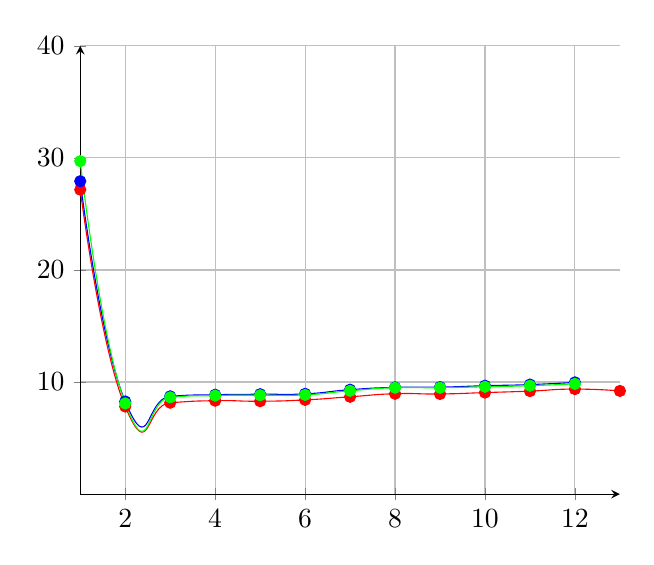
\begin{tikzpicture}
\begin{axis}[axis lines=middle, grid=both, ymin=0, ymax=40]\addplot [red, smooth, tension=1, mark=*] coordinates {(1, 27.164)(2, 7.814)(3, 8.156)(4, 8.338)(5, 8.291)(6, 8.409)(7, 8.685)(8, 8.955)(9, 8.938)(10, 9.06)(11, 9.193)(12, 9.371)(13, 9.207)};
\addplot [blue, smooth, tension=1, mark=*] coordinates {(1, 27.921)(2, 8.266)(3, 8.725)(4, 8.868)(5, 8.914)(6, 8.948)(7, 9.319)(8, 9.525)(9, 9.549)(10, 9.674)(11, 9.775)(12, 9.971)};
\addplot [green, smooth, tension=1, mark=*] coordinates {(1, 29.708)(2, 8.096)(3, 8.635)(4, 8.794)(5, 8.824)(6, 8.856)(7, 9.217)(8, 9.49)(9, 9.492)(10, 9.581)(11, 9.674)(12, 9.841)};
\end{axis}
\end{tikzpicture}
\end{document}